\documentclass[11pt]{article}
\usepackage[a4paper,margin=1in]{geometry}
\usepackage{amsmath,amssymb,amsthm,mathtools}
\usepackage{booktabs}
\usepackage{graphicx}
\usepackage{hyperref}
\usepackage[nameinlink,capitalise]{cleveref}
\usepackage[numbers,sort&compress]{natbib}

\newtheorem{theorem}{Theorem}[section]
\newtheorem{proposition}[theorem]{Proposition}
\newtheorem{corollary}[theorem]{Corollary}
\theoremstyle{remark}
\newtheorem{remark}[theorem]{Remark}
\newcommand{\norm}[1]{\left\lVert#1\right\rVert}

\title{Trace-Normalized Late-Memory Packets\\
\large A Gap-Free Dynamic Gramian and the Failure of Angle Perturbation}
\author{Liang Wang}
\date{July 2026}

\begin{document}
\maketitle

\begin{abstract}
RH-85 showed that a clock-rank packet built from a strict-prefix snapshot can
capture the terminal postblock state, while the unweighted prefix Gramian can
retain large transient energy.  This paper replaces the isolated snapshot by
an online, scale-free late-memory statistic.

For $X_t=A^tS$ and $0\le\eta<1$, define
\[
 G_j=\frac{X_j^*X_j}{\norm{X_j}_2^2}+\eta G_{j-1},\qquad G_{-1}=0.
\]
The normalized-memory variational theorem identifies the leading rank-$r$
projection of $G_j$ as the minimizer of the exponentially weighted sum of
relative snapshot residuals.  The associated stacked tail bounds the current
relative residual without any singular-value gap.  RH-85 then propagates the
packet through the unused suffix.  This is a gap-free energy transfer, not a
principal-angle argument.

At all five archived scales, one universal value $\eta=1/512$ and packet time
$\lceil2M/3\rceil$ give a direct 192-bit terminal residual below
$1.10\times10^{-5}$ and captured energy above $0.99999999988$.  Less than
$0.196\%$ of the normalized trace memory precedes the current snapshot.  The
weighted packet improves the raw unweighted prefix residual by at least three
orders of magnitude and by more than $4.6\times10^6$ in the strongest case.

Conversely, every standard perturbation-to-gap ratio for comparing the memory
packet to the point packet exceeds $8.9\times10^6$, reaching above
$8.1\times10^9$.  Thus the angle perturbation route is quantitatively unusable
at the anchors even though captured energy is stable.  Uniform weighted
Rayleigh leakage, Stage A, Hilbert--Polya, and the Riemann Hypothesis remain
open.
\end{abstract}

\noindent\textbf{Keywords:} dynamic Gramian; exponential forgetting;
captured energy; principal angles; effective rank; interval arithmetic.

\medskip
\noindent\textbf{MSC 2020:} 47A75; 47B10; 15A18; 65G20.

\section{A scale-free late-memory statistic}

RH-84 isolated captured energy as the minimal effective-rank invariant
\citep{WangKyFan2026}.  RH-85 then proved snapshot transfer and found a strong
strict-prefix packet, but also gave an explicit no-go theorem for unweighted
prefix energy \citep{WangSnapshot2026}.  The problem is amplitude: a large
early transient can dominate $\sum_{t\le j}X_t^*X_t$ long after it has become
irrelevant to the terminal state.

Normalize every nonzero snapshot by its Hilbert--Schmidt norm and forget the
past geometrically.  Define the stacked operator
\[
 \mathcal N_{\eta,j}u=
 \left(\eta^{(j-t)/2}\frac{X_tu}{\norm{X_t}_2}\right)_{t=0}^j.
\]
Its Gramian is exactly $G_j=\mathcal N_{\eta,j}^*\mathcal N_{\eta,j}$ and
satisfies the online recursion in the abstract.

\section{Gap-free variational and transfer theorems}

\begin{theorem}[Normalized-memory variational theorem]
\label{thm:variational}
Let $P_{\eta,j,r}$ be the leading rank-$r$ spectral projection of $G_j$.
Then
\begin{align}
 \tau_r(\mathcal N_{\eta,j})^2
 &=\min_{\operatorname{rank}P=r}
 \sum_{t=0}^j\eta^{j-t}
 \frac{\norm{X_t(I-P)}_2^2}{\norm{X_t}_2^2},
 \label{eq:objective}\\
 \frac{\norm{X_j(I-P_{\eta,j,r})}_2}{\norm{X_j}_2}
 &\le \tau_r(\mathcal N_{\eta,j}).
 \label{eq:current}
\end{align}
No spectral gap is required.
\end{theorem}

\begin{proof}
The objective in \eqref{eq:objective} equals
$\norm{\mathcal N_{\eta,j}(I-P)}_2^2$.  Ky Fan's principle and
Eckart--Young identify its minimizer with the leading spectral projection of
$G_j$ \citep{Bhatia1997}.  The $t=j$ summand has weight one and is bounded by
the full nonnegative sum, proving \eqref{eq:current}.
\end{proof}

\begin{corollary}[Gap-free energy transfer]
\label{cor:transfer}
For $j\le M$,
\begin{equation}
 \frac{\norm{X_M(I-P_{\eta,j,r})}_2}{\norm{X_M}_2}
 \le
 \frac{\norm{A^{M-j}}\norm{X_j}_2}{\norm{X_M}_2}
 \tau_r(\mathcal N_{\eta,j}).
 \label{eq:transfer}
\end{equation}
\end{corollary}

\begin{proof}
Apply the RH-85 snapshot transfer theorem to \eqref{eq:current}.
\end{proof}

The total normalized trace memory is
$(1-\eta^{j+1})/(1-\eta)$.  Hence the mass before the current snapshot is at
most $\eta/(1-\eta)$.  This deterministic bound prevents raw amplitude from
overriding the intended time localization.

\section{Why principal-angle control is the wrong gate}

Write $\widehat G_j=X_j^*X_j/\norm{X_j}_2^2$ and
$E_j=G_j-\widehat G_j$.  A Davis--Kahan route would compare spectral
projections using $\norm{E_j}/\delta_{j,r}$, where
$\delta_{j,r}=\lambda_r(\widehat G_j)-\lambda_{r+1}(\widehat G_j)$
\citep{StewartSun1990}.  At a nearly finite-rank tail this gap can be much
smaller than every physically relevant energy tolerance.  The ratio may then
be enormous although both packets capture essentially the same energy.

This does not contradict perturbation theory.  It says only that identifying
individual low-energy directions is much harder than bounding the total
energy left outside a packet.  The latter is exactly the invariant required
by RH-84.

\section{Five-scale 192-bit audit}

We use $\eta=1/512$, $j=\lceil2M/3\rceil$, and
$r=\lceil H_\sigma\rceil+2$.  The packet is computed from the binary64 memory
Gramian.  Its snapshot and terminal residuals are then evaluated directly in
192-bit Arb arithmetic after exact binary lifting.  The rank bound remains
exact, and the Frobenius suffix inequality is interval certified.

\begin{table}[ht]
\centering
\small
\begin{tabular}{rrrrr}
\toprule
$\sigma$ & rank & worst weighted tail & worst unweighted tail & min gap ratio\\
\midrule
0.16 & 4 & $1.10\times10^{-5}$ & $1.38\times10^{-1}$ & $1.85\times10^7$\\
0.08 & 5 & $2.0\times10^{-7}$ & $1.10\times10^{-1}$ & $8.98\times10^6$\\
0.04 & 6 & $3.0\times10^{-7}$ & $2.45\times10^{-1}$ & $9.87\times10^6$\\
0.02 & 6 & $3.0\times10^{-7}$ & $2.84\times10^{-1}$ & $4.00\times10^9$\\
0.01 & 7 & $2.0\times10^{-7}$ & $3.26\times10^{-1}$ & $3.32\times10^9$\\
\bottomrule
\end{tabular}
\caption{Worst channel tails and the smaller directional gap ratio at each
scale.  Tail values are rounded conservatively from the generated audit.}
\label{tab:audit}
\end{table}

The weighted packet is close to the point packet in captured energy, but not
certifiably close in principal angle.  The minimum gap ratio exceeds one
million by a wide margin at every anchor.  Meanwhile the normalized past
trace fraction is below $0.001954$ independently of the ambient dimension.

\begin{figure}[ht]
\centering
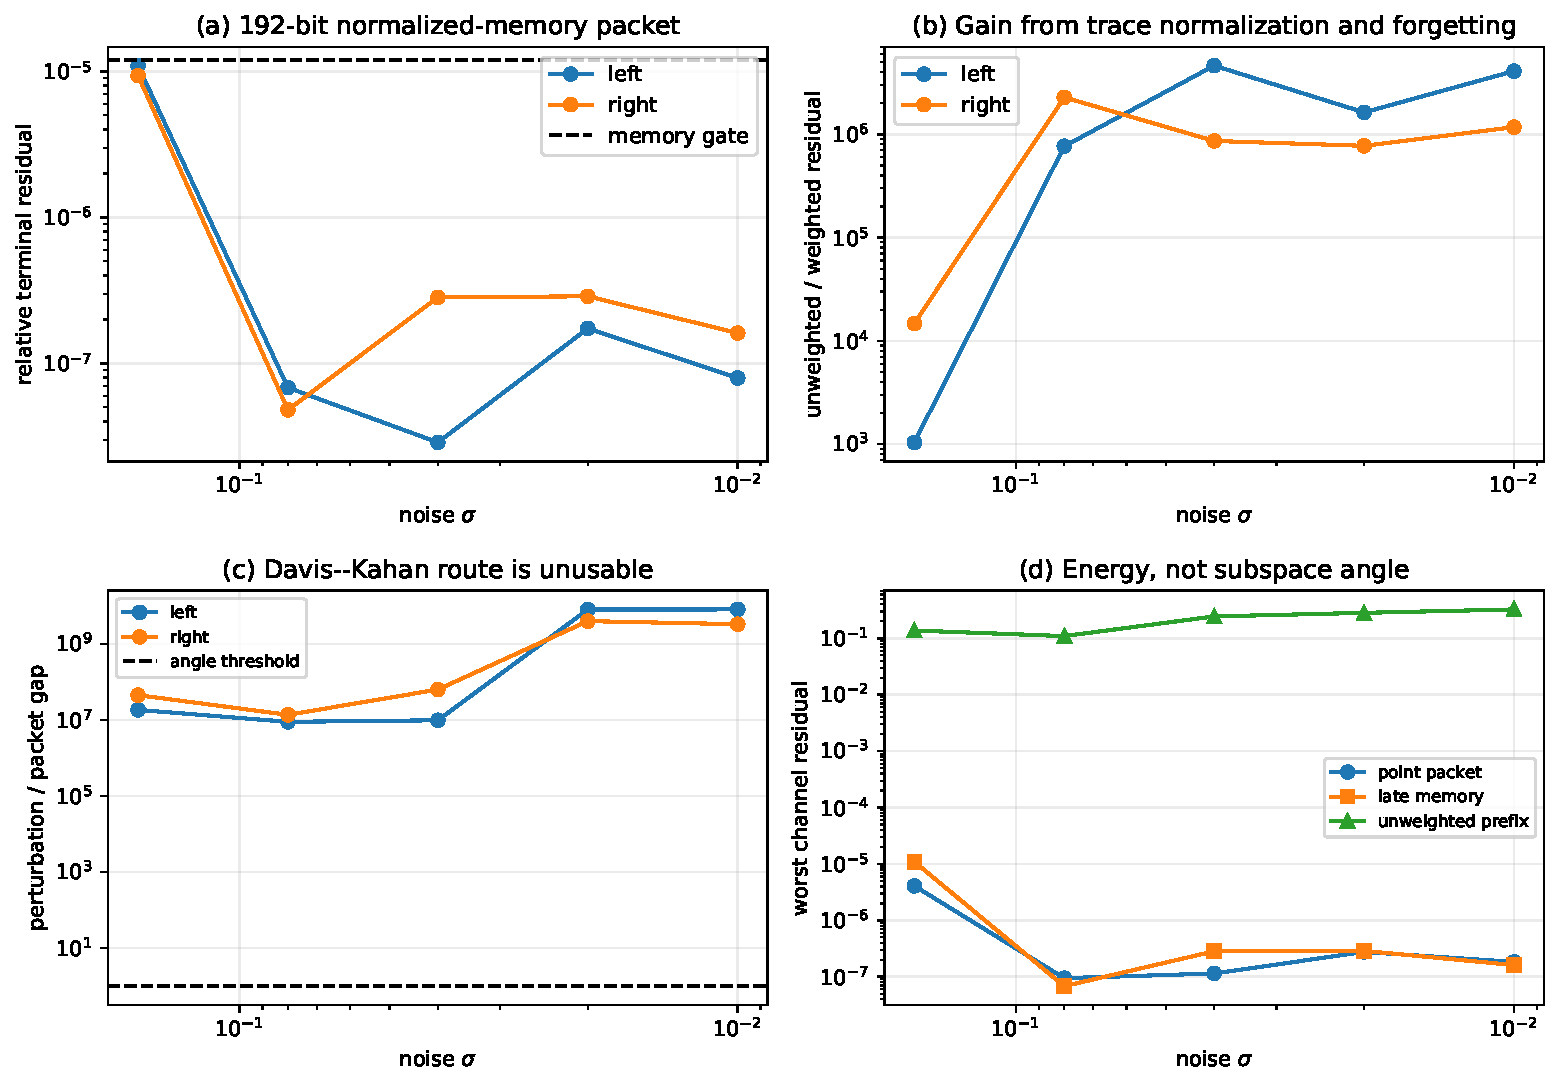
\includegraphics[width=\textwidth]{figures/trace_normalized_late_memory.pdf}
\caption{Interval late-memory residuals, improvement over raw prefix energy,
the failure of gap-based angle control, and the three packet choices.}
\label{fig:audit}
\end{figure}

\section{Boundary and next theorem}

The durable object is now the weighted Rayleigh leakage in
\eqref{eq:objective}.  An all-level proof may bound it directly through a
one-block energy recursion, without resolving unstable tail eigenspaces.  A
representative next target is a packet-energy drift inequality comparing
$\operatorname{tr}(P_jG_{j+1})$ with $\operatorname{tr}(P_jG_j)$ plus a
controlled injection term.

RH-86 proves the variational and transfer statements and validates the frozen
late-memory packets.  It does not derive $\eta$ from the continuum dynamics,
prove all-level weighted leakage, close Stage A1 or Stage A4, construct a
relative fixed-disk determinant or self-adjoint Hilbert--Polya operator,
identify zeta zeros, or prove the Riemann Hypothesis.

\bibliographystyle{plainnat}
\bibliography{references}

\end{document}
